\documentclass{eecslides}\usepackage[]{graphicx}\usepackage[]{color}
%% maxwidth is the original width if it is less than linewidth
%% otherwise use linewidth (to make sure the graphics do not exceed the margin)
\makeatletter
\def\maxwidth{ %
  \ifdim\Gin@nat@width>\linewidth
    \linewidth
  \else
    \Gin@nat@width
  \fi
}
\makeatother

\definecolor{fgcolor}{rgb}{0.345, 0.345, 0.345}
\newcommand{\hlnum}[1]{\textcolor[rgb]{0.686,0.059,0.569}{#1}}%
\newcommand{\hlstr}[1]{\textcolor[rgb]{0.192,0.494,0.8}{#1}}%
\newcommand{\hlcom}[1]{\textcolor[rgb]{0.678,0.584,0.686}{\textit{#1}}}%
\newcommand{\hlopt}[1]{\textcolor[rgb]{0,0,0}{#1}}%
\newcommand{\hlstd}[1]{\textcolor[rgb]{0.345,0.345,0.345}{#1}}%
\newcommand{\hlkwa}[1]{\textcolor[rgb]{0.161,0.373,0.58}{\textbf{#1}}}%
\newcommand{\hlkwb}[1]{\textcolor[rgb]{0.69,0.353,0.396}{#1}}%
\newcommand{\hlkwc}[1]{\textcolor[rgb]{0.333,0.667,0.333}{#1}}%
\newcommand{\hlkwd}[1]{\textcolor[rgb]{0.737,0.353,0.396}{\textbf{#1}}}%
\let\hlipl\hlkwb

\usepackage{framed}
\makeatletter
\newenvironment{kframe}{%
 \def\at@end@of@kframe{}%
 \ifinner\ifhmode%
  \def\at@end@of@kframe{\end{minipage}}%
  \begin{minipage}{\columnwidth}%
 \fi\fi%
 \def\FrameCommand##1{\hskip\@totalleftmargin \hskip-\fboxsep
 \colorbox{shadecolor}{##1}\hskip-\fboxsep
     % There is no \\@totalrightmargin, so:
     \hskip-\linewidth \hskip-\@totalleftmargin \hskip\columnwidth}%
 \MakeFramed {\advance\hsize-\width
   \@totalleftmargin\z@ \linewidth\hsize
   \@setminipage}}%
 {\par\unskip\endMakeFramed%
 \at@end@of@kframe}
\makeatother

\definecolor{shadecolor}{rgb}{.97, .97, .97}
\definecolor{messagecolor}{rgb}{0, 0, 0}
\definecolor{warningcolor}{rgb}{1, 0, 1}
\definecolor{errorcolor}{rgb}{1, 0, 0}
\newenvironment{knitrout}{}{} % an empty environment to be redefined in TeX

\usepackage{alltt}
\mode<presentation>
%\usecolortheme{BBSDark}

%%------------------
% Language and font
\usepackage[english]{babel}
\usepackage[utf8]{inputenc}

%%------------------
\usepackage{graphicx}
\usepackage{color}
\usepackage{tikz}
\usetikzlibrary{calc, shapes, backgrounds, arrows}

% --- include packages
\usepackage{subfigure}
\usepackage{multicol}
\usepackage{amsthm}
\usepackage{mathrsfs}
\usepackage{amsmath}
\usepackage{amssymb}
\usepackage{enumitem}

% --- Writing certain lines in courrier 
\usepackage{courier}

%%------------------
\DeclareRobustCommand\refmark[1]{\textsuperscript{\ref{#1}}}

%%------------------ Tune the template
\setbeamertemplate{blocks}[rounded][shadow=false]

\title[Day 3]{Markov Chain Monte Carlo (MCMC) and Model Evaluation}
\vspace{0.4cm}
\vspace{0.6cm}

%%% Begin slideshow
\IfFileExists{upquote.sty}{\usepackage{upquote}}{}
\begin{document}

\begin{frame}
  \titlepage
\end{frame}

\section{Intro}


\frame{
\frametitle{Ecological context}
\framesubtitle{How important is elevation in defining sugar maple distribution on mont Sutton?}


\begin{columns}[T]
\begin{column}{0.6\textwidth}

Mont Sutton

\vspace{-0.7cm}

  \begin{center}
    \scalebox{0.2}{
      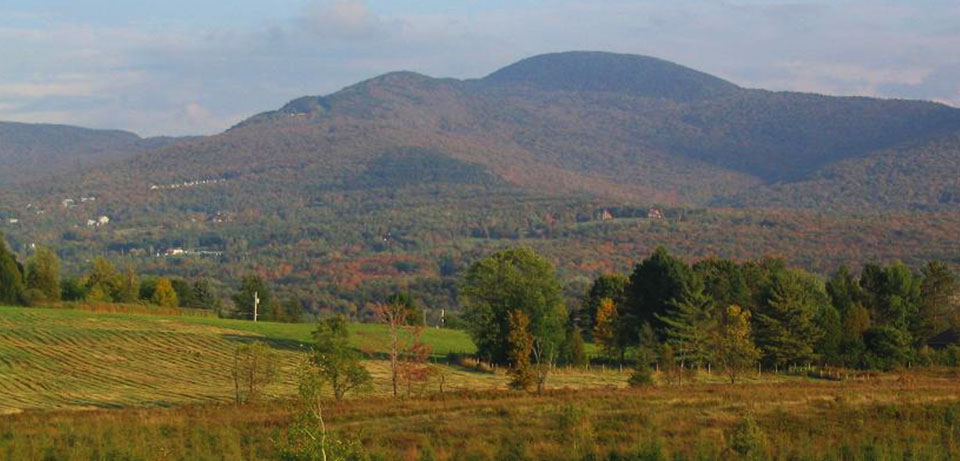
\includegraphics{Image/Mont_Sutton.jpg}
    }
  \end{center}

  \vspace{-0.2cm}
  
  {\large\bf Model}
  
  \vspace{-0.5cm}
  
  {\large $$P(y=1) = \beta x + \epsilon$$}

  \vspace{-0.8cm}

 where
 \begin{itemize}
  \item[$y$] is the distribution of sugar maple
  \item[$x$] is elevation
  \textcolor{red}{\large\item[$\beta$] is the importance of elevation}
  \item[$\epsilon$] is the model residuals
 \end{itemize}
\end{column}
\begin{column}{0.5\textwidth}
\vspace{-0.5cm}
\begin{knitrout}
\definecolor{shadecolor}{rgb}{0.969, 0.969, 0.969}\color{fgcolor}
\includegraphics[width=\maxwidth]{figure/acerSacc-1} 

\end{knitrout}
\end{column}
\end{columns}
}

\frame{
\frametitle{Linking Frequentist and Bayesian Statistics}
\framesubtitle{How can we estimate model parameters and what does it imply?}

{\Large\bf Frequentist}

\vspace{0.1cm}

%Want to find the best model parameter(s) ($\beta$) for the data at hand (sugar maple distribution)
Want to find the best model parameter(s) for the data at hand

{\Large 
	$$\textcolor{blue}{\text{Likelihood}}\hspace{1.5cm}P(\text{Data}|\text{Model})$$
}

{\large They are interested in {\bf maximizing} the \textcolor{blue}{\text{Likelihood}}}

\vspace{0.1cm}

{\large They need data}

\vspace{0.2cm}

{\bf This can be done using}

\begin{itemize}
  \item Simulated annealing
  \item The Nelder-Mead Simplex
  \item Minimizing the sums of squares
  \item \dots
\end{itemize}
}

\frame{
\frametitle{Linking Frequentist and Bayesian Statistics}
\framesubtitle{How can we estimate model parameters and what does it imply?}

{\Large\bf Bayesian}

\vspace{0.1cm}

%Want to find how good the model parameter(s) ($\beta$) given some data (sugar maple distribution)
Want to find how good the model parameter(s) are given some data

{\Large 
	$$\textcolor{orange}{\text{Posterior}}\hspace{1.5cm}P(\text{Model}|\text{Data})$$
}

{\large They are intered in the \textcolor{orange}{\text{posterior}} distribution}

\vspace{0.1cm}

{\large They need data and prior information}

\vspace{0.2cm}

{\large\bf Recall that}

{\Large 
	$$\underbrace{P(\text{Model}|\text{Data})}_{\textcolor{orange}{Posterior}}\propto \underbrace{P(\text{Data}|\text{Model})}_\text{\textcolor{blue}{Likelihood}}\underbrace{P(\text{Model})}_\text{\textcolor{green!50!black}{Prior}}$$
}

}

\frame{
\frametitle{Bayesian Statistics}
\framesubtitle{A few words about the prior}

{\Large Definition of prior probability}

\vspace{0.1cm}

The {\bf prior probability} informes us about the probability of the model being true \textit{before} the current data is considered.

\vspace{0.5cm}

{\Large Types of priors}

\vspace{0.1cm}

{\bf\large Uninformative}

\vspace{0.1cm}

These priors are meant to bring very little information about the model

\vspace{0.1cm}

{\bf\large Informative}

\vspace{0.1cm}

These priors bring information about the model that is available

}

\frame{
\frametitle{Bayesian Statistics}
\framesubtitle{A few words about the prior}

{\Large\bf Uninformative priors}

\vspace{0.1cm}

{\bf Example:} If we have no idea of how elevation influence sugar maple

\vspace{0.1cm}

{\bf Gaussian distribution}

\vspace{0.1cm}

\begin{columns}
\begin{column}{0.5\textwidth}
\large $$\frac{1}{\sqrt{2\pi\sigma^2}}e^{-\frac{(x-\mu)^2}{2\sigma^2}}$$
\end{column}
with
\begin{column}{0.5\textwidth}
\begin{itemize}
  \item $\mu = 0$
  \item $\sigma = \text{Large say 100}$
\end{itemize}
\end{column}
\end{columns}

\vspace{0.2cm}
\begin{knitrout}
\definecolor{shadecolor}{rgb}{0.969, 0.969, 0.969}\color{fgcolor}
\includegraphics[width=\maxwidth]{figure/uninfoPrior-1} 

\end{knitrout}

}

\frame{
\frametitle{Bayesian Statistics}
\framesubtitle{A few words about the prior}

{\Large\bf Informative priors}

\vspace{0.1cm}

{\bf Example:} If we know that 
\begin{itemize}
  \item There are less sugar maples the higher we go
  \item The influence of elevation on sugar maple cannot be more than two folds
\end{itemize}

\vspace{0.1cm}

{\bf Uniform distribution}

\vspace{0.1cm}

\begin{columns}
\begin{column}{0.5\textwidth}
\large $$\left\{
  \begin{array}{cl}
    \frac{1}{b-a} & \text{for } x\in [a,b]\\
    0 &\text{otherwise}\\
  \end{array}
\right.$$
\end{column}
with
\begin{column}{0.5\textwidth}
\begin{itemize}
  \item $a > -2$
  \item $b < 0$
\end{itemize}
\end{column}
\end{columns}

\vspace{0.2cm}
\begin{knitrout}
\definecolor{shadecolor}{rgb}{0.969, 0.969, 0.969}\color{fgcolor}
\includegraphics[width=\maxwidth]{figure/infoPrior-1} 

\end{knitrout}
}


\section{Bayesian}

\frame{
\frametitle{Bayesian Statistics}
\framesubtitle{Estimating model parameters}

{\large\bf When the likelihood \textit{can} be solved analytically}

Start from Dominique's day 2 work.

%\vspace{0.2cm}

%{\bf Example}

%\vspace{0.1cm}

%Assuming that the sugar maple follows a binomial distribution where

%\begin{itemize}[leftmargin=2cm]
%  \item[Data:] $y$
%  \item[Model ($\theta$):] $\beta x$
%\end{itemize}
%then the \textcolor{blue}{likelihood} is
%\begin{align*}
%  P(y|\theta)&=\binom{1}{y}\theta^y\left(1-\theta\right)^{1-y}\\
%  &\propto\theta^y\left(1-\theta\right)^{1-y}\\
%  &\propto\left(\beta x\right)^y\left(1-\beta x\right)^{1-y}\\
%\end{align*}


}

\frame{
\frametitle{Bayesian Statistics}
\framesubtitle{Estimating $\beta$}
Exercice (by hand?)
}

\frame{
\frametitle{Bayesian Statistics}
\framesubtitle{Estimating $\beta$}

{\Large When the likelihood {\bf cannot} be solved analytically (Difficult problem)}

Talk about MCMC
Mention that MCMC {\bf can} be used for simple problems but it is generally time consumming so generally not the best way to go
}

\section{MCMC}

\frame{
\frametitle{Properties Markov Chain Monte Carlo (MCMC)}

{\large\bf Similarity with simulated annealing}
\begin{itemize}
  \item New parameter values are chosen sequentially but randomly
  \item There are many ways to choose and accept new parameter values
\end{itemize}

\vspace{0.2cm}

{\large\bf Difference with simulated annealing}
\begin{itemize}
  \item The main goal of MCMC is to sample the \textcolor{orange}{posterior} distribution
  \item No ``temperature'' is defined
  \item It is impossible to get stuck in a loop while iterating
\end{itemize}

\vspace{0.2cm}

{\large\bf Assumptions of MCMC}

\begin{itemize}
  \item All potential parameter combinations can be reached from all other parameter combination
  \item After enough iterations the chain will converges to a stationary distribution
\end{itemize}
}

\section{MH}

\frame{
\frametitle{The Metropolis-Hasting Algorithm}
\framesubtitle{Theory}
\large
{\bf Usefulness}
\begin{itemize}
  \item It is an MCMC well designed to approach univariate problems
  \item It is useful to sample Bayesian posterior distribution
\end{itemize}

{\bf Properties}
\begin{itemize}
  \item Each iteration generates a sample from the target distribution
  \item Samples are dependent on one another (they are autocorrelated)... So effective sample size is smaller than the chain length
\end{itemize}
}


\frame{
\frametitle{The Metropolis-Hasting Algorithm}
\framesubtitle{How the Metropolis-Hasting Algorithm works}

{\Large\bf Defining the important parts}

\vspace{0.2cm}

\begin{itemize}
  \item {\large Number of steps ($N$) to run the MCMC}

  \vspace{0.2cm}

  \hspace{0.2cm} It has to be large. For example, 5000 steps

  \vspace{0.2cm}
  
  \item {\large Starting value ($\theta$)}

  \vspace{0.2cm}

  \hspace{0.2cm} It should roughly describe the distribution to be estimated 

  \vspace{0.2cm}
  
  \item {\large Target distribution ($f(\theta)$)}

  \vspace{0.2cm}

  \hspace{0.2cm} It is the distribution of value we aim at estimating
  
  \vspace{0.2cm}

  \item {\large Jumping distribution ($j(\theta_{cand}|\theta_{t-1})$)}

  \vspace{0.2cm}
  
  \hspace{0.2cm} Many choices are possible but it must allow for positive recurrence

  \vspace{0.2cm}
  
  \hspace{0.2cm} The normal distribution ($\mu$ = $\theta_{cand}$, $\sigma^2$ = 1) is a good starting point
     $$\frac{1}{\sqrt{2\pi\sigma^2}}e^{-\frac{(x-\mu)^2}{2\sigma^2}}$$
  

\end{itemize}
}


\frame{
\frametitle{The Metropolis-Hasting Algorithm}
\framesubtitle{How the Metropolis-Hasting Algorithm works}

{\Large\bf Defining the important parts (conitnued)}

\vspace{0.2cm}

\begin{itemize}
  \item {\large Acceptance probability}
  $$r=\frac{f(\theta_{cand})j(\theta_{t-1}|\theta_{cand})}{f(\theta_{t-1})j(\theta_{cand}|\theta_{t-1})}$$
\end{itemize}

\vspace{1cm}

Note that for any \textit{symmetric} distribution, such as the uniform distribution, the acceptance probability becomes
$$r=\frac{f(\theta_{cand})}{f(\theta_{t-1})}$$
This is known as the \textbf{Metropolis algorithm}
}
\frame{
\frametitle{The Metropolis-Hasting Algorithm}
\framesubtitle{How the Metropolis-Hasting Algorithm works conceptually}

\bf

{\Large Algorithm in \texttt{pseudocode}}

\vspace{0.4cm}

\texttt{for t in 1 to N}

\vspace{0.2cm}

\hspace{0.5cm}\texttt{sample theta\_c from j(theta\_c|theta[t-1])}
  
\vspace{0.2cm}

\hspace{0.5cm}\texttt{set r\_cand = r(theta\_c, theta[t-1])}
  
\vspace{0.2cm}

\hspace{0.5cm}\texttt{sample U from uniform(0, 1)}
  
\vspace{0.2cm}

\hspace{0.5cm}\texttt{IF U < r\_cand}

\vspace{0.2cm}

\hspace{1cm}\texttt{theta[t] = theta\_c}

\vspace{0.2cm}

\hspace{0.5cm}\texttt{ELSE}

\vspace{0.2cm}

\hspace{1cm}\texttt{theta[t] = theta[t-1]}

}

\section{Good Practices}

\frame{
\frametitle{Good Practices}
\framesubtitle{Chain length}

{\large\bf A rough procedure to decide how many steps is enough}

\begin{itemize}
  \item[{\bf Step 1}] Perform a pilot run for a reduced number of steps (10 to 100) and measure the time it takes
  \item[{\bf Step 2}] Decide on a number of steps to run the algorithm to obtain a result in a reasonable amount of time
  \item[{\bf Step 3}] Run the algorithm again !
  \item[{\bf Step 4}] Study the chain visually
\end{itemize}

\vspace{0.2cm}

{\large\bf The Raftery-Lewis diagnostic}

\vspace{0.2cm}

It relies on a pilot run to estimate the number of steps to be carried out

\vspace{0.1cm}

It is implemented in the \texttt{raftery.diag} function of the \texttt{coda} R package

}

\frame{
\frametitle{Good Practices}
\framesubtitle{Trace plot}

\begin{knitrout}
\definecolor{shadecolor}{rgb}{0.969, 0.969, 0.969}\color{fgcolor}
\includegraphics[width=\maxwidth]{figure/trace-1} 

\end{knitrout}
}

\frame{
\frametitle{Good Practices}
\framesubtitle{Thinning}

\large

Thinning is essentially {\bf subsampling}

\vspace{-0.5cm}

\begin{knitrout}
\definecolor{shadecolor}{rgb}{0.969, 0.969, 0.969}\color{fgcolor}
\includegraphics[width=\maxwidth]{figure/thining1-1} 

\end{knitrout}

If we ran the same MCMC as above but instead for 50000 steps and we save the $\theta$ at every 10 steps, we obtain

\vspace{-0.2cm}

\begin{knitrout}
\definecolor{shadecolor}{rgb}{0.969, 0.969, 0.969}\color{fgcolor}
\includegraphics[width=\maxwidth]{figure/thining2-1} 

\end{knitrout}

}

\frame{
\frametitle{Good Practices}
\framesubtitle{Burn-in}

\large

Burn-in is throwing away some iterations at the beginning of the MCMC run 

\vspace{-0.5cm}

\begin{knitrout}
\definecolor{shadecolor}{rgb}{0.969, 0.969, 0.969}\color{fgcolor}
\includegraphics[width=\maxwidth]{figure/burnin1-1} 

\end{knitrout}

After burn-in, we obtain

\vspace{-0.2cm}

\begin{knitrout}
\definecolor{shadecolor}{rgb}{0.969, 0.969, 0.969}\color{fgcolor}
\includegraphics[width=\maxwidth]{figure/burnin2-1} 

\end{knitrout}

}


\frame{
\frametitle{Exercice}
\framesubtitle{Write your own Metropolis-Hasting Algorithm}


}

\section{Convergence}

\frame{
\frametitle{Convergence}
\framesubtitle{Multiple chains}
\large
Rerun the estimation procedure multiple time with different starting values

\begin{knitrout}
\definecolor{shadecolor}{rgb}{0.969, 0.969, 0.969}\color{fgcolor}
\includegraphics[width=\maxwidth]{figure/multChain-1} 

\end{knitrout}
}


\frame{
\frametitle{Convergence}
\framesubtitle{Density plot}
\large

\begin{knitrout}
\definecolor{shadecolor}{rgb}{0.969, 0.969, 0.969}\color{fgcolor}
\includegraphics[width=\maxwidth]{figure/densPlot-1} 

\end{knitrout}
}

\frame{
\frametitle{Convergence}
\framesubtitle{Geweke convergence diagnostics}
{\bf It compares two sections of the same chain}

\vspace{0.2cm}

Technically, it is two sample $t$ test of mean with unequal variance 

{\large $$Z = \frac{\bar\theta_A-\bar\theta_B}{\sqrt{\frac{S_A}{n_A}+\frac{S_B}{n_B}}}$$}

\vspace{-0.5cm}

where

\vspace{0.2cm}

$\bar\theta_A$ and $\bar\theta_B$ are the means of the chain section $\theta_A$ and $\theta_B$,

$n_A$ and $n_B$ are the number of steps of the chain section $\theta_A$ and $\theta_B$,

\vspace{0.2cm}

\begin{columns}
  \begin{column}{0.5\textwidth}
$$S_A = \frac{\sigma_A^2}{(1-\sum\alpha_A)^2}$$
  \end{column}
  \begin{column}{0.5\textwidth}
$$S_B = \frac{\sigma_B^2}{(1-\sum\alpha_B)^2}$$
  \end{column}
\end{columns}

\vspace{0.2cm}

$\sigma_A$ and $\sigma_B$ are the variance of the chains sections $\theta_A$ and $\theta_B$

$\alpha_A$ and $\alpha_B$ are autoregressive parameters of the chain sections $\theta_A$ and $\theta_B$ 

\vspace{0.5cm}

It is implemented in the \texttt{geweke.diag} function of the \texttt{coda} R package
}

\frame{
\frametitle{Convergence}
\framesubtitle{Gelman-Rubin convergence diagnostics}
\footnotesize
{\bf It compares multiple chains}

\vspace{0.2cm}

it is a corrected ratio of the pooled variance of all chains with the within variance of each chain

$$R=\sqrt{\frac{V}{W}}$$

\vspace{0.2cm}

{\bf Chains pooled variance}
$$V=\frac{N-1}{N}W+\frac{1}{N}B$$
where 
$$B=\frac{N}{M-1}\sum_{m=1}^M(\bar\theta_m-\bar\theta)^2,$$
$N$ is the length of each chain (it is assumed to be the same)

$M$ is the number of chains

$\bar\theta_m$ is the mean chain $m$,

$\bar\theta$ is the mean of all chains.

\vspace{0.2cm}

{\bf Within chain variance}
$$W=\frac{1}{M}\sum_{m=1}^M\sigma^2$$

\vspace{-0.1cm}

It is implemented in the \texttt{gelman.diag} function of the \texttt{coda} R package.
}

\section{MH (more)}

\frame{
\frametitle{Adaptive Metropolis-Hasting Algorithm}

\large

We adapt the standard deviation of the normal distribution during burn-in 

{\Large $$\frac{1}{\sqrt{2\pi\sigma^2A}}e^{-\frac{(x-\mu)^2}{2\sigma^2A}}$$}

\vspace{0.1cm}

where $A$ is a tuning parameter

}

\frame{
\frametitle{Adaptive Metropolis-Hasting Algorithm}
\bf
{\large Adaptative Algorithm in \texttt{pseudocode}}

\vspace{0.1cm}

\textcolor{orange}{\texttt{set A = 1}}

\texttt{for t in 1 to N}

\hspace{0.5cm}\texttt{sample theta\_c from j(theta\_c|theta[t-1]\textcolor{orange}{, A})}
  
\hspace{0.5cm}\texttt{set r\_cand = r(theta\_c, theta[t-1])}
  
\hspace{0.5cm}\texttt{sample U from uniform(0, 1)}

\hspace{0.5cm}\texttt{IF U < r\_cand}

\hspace{1cm}\texttt{theta[t] = theta\_c}

\textcolor{orange}{\hspace{1cm}\texttt{IF burning}}

\textcolor{orange}{\hspace{1.5cm}\texttt{A = A * 1.01}}

\hspace{0.5cm}\texttt{ELSE}

\hspace{1cm}\texttt{theta[t] = theta[t-1]}

\textcolor{orange}{\hspace{1cm}\texttt{IF burning}}

\textcolor{orange}{\hspace{1.5cm}\texttt{A = A / 1.01}}
}

\frame{
\frametitle{Exercice}
\framesubtitle{Build your own adaptive Metropolis-Hasting algorithm}

}


\frame{
\frametitle{Single component adaptive Metropolis-Hasting algorithm}

{\large Adaptative Algorithm in \texttt{pseudocode}}

\footnotesize
{\bf

\vspace{0.2cm}

\texttt{set A = \textcolor{orange}{repeat(1,nparam)}}

\texttt{for t in 1 to N}

\textcolor{orange}{\hspace{0.5cm}\texttt{for i in 1 to nparam}}

\hspace{1cm}\texttt{sample theta\_c\textcolor{orange}{[i]} from j(theta\_c\textcolor{orange}{[i]}|theta[\textcolor{orange}{i,}t-1], A[i])}
  
\hspace{1cm}\texttt{set r\_cand = r(theta\_c, theta[t-1])}
  
\hspace{1cm}\texttt{sample U from uniform(0, 1)}

\hspace{1cm}\texttt{IF U < r\_cand}

\hspace{1.5cm}\texttt{theta[t] = theta\_c}

\hspace{1.5cm}\texttt{IF burning}

\hspace{2cm}\texttt{A\textcolor{orange}{[i]} = A\textcolor{orange}{[i]} * 1.01}

\hspace{1cm}\texttt{ELSE}

\hspace{1.5cm}\texttt{theta[t] = theta[t-1]}

\hspace{1.5cm}\texttt{IF burning}

\hspace{2cm}\texttt{A\textcolor{orange}{[i]} = A\textcolor{orange}{[i]} / 1.01}
}

\vspace{0.2cm}

\begin{itemize}
  \item The SCAM is designed for models with multiple parameters
  \item {\bf \texttt{theta\_cand}} is a vector, not a single value
  \item {\bf \texttt{theta}} is a matrix, not a vector
\end{itemize}
}

\frame{
\frametitle{Exercice}
\framesubtitle{Build your own single component adaptive Metropolis-Hasting algorithm}

}

\section{Gibbs}

\frame{
\frametitle{Gibbs Sampling}
\framesubtitle{Properties}

\large

\begin{itemize}
  \item A specific case of the single component Metropolis-Hasting algorithm
  
  \vspace{0.5cm}
  
  \item It is designed to sample from a posterior with multiple parameters
  
  $$p(\theta_1, \theta_2, \dots, \theta_p|y,\mathbf{X})$$
  
  \vspace{0.25cm}
  
  \item For each step, the Gibb sampler cycles through the $p$ parameters of $\theta$ where a sample is taken conditional on all other $p-1$ parameters

  $$f(\theta_i|y,\mathbf{X}, \theta_1, \dots, \theta_i, \dots, \theta_p)$$
  
\end{itemize}

}


\frame{
\frametitle{Gibbs Sampling}
\framesubtitle{Properties}

{\Large\bf Defining the (additional) important parts}

\begin{itemize}
  \item {\large Input data}

  \vspace{0.2cm}

  \hspace{0.2cm} This includes both the dependent and the independent variables

  \vspace{0.2cm}
  
  \item {\large Define the joint posterior distributoin}
  
  $$f(\text{Model},\text{Data})$$
  
  \item {\large Define the model (and thus the number of parameters) in the posterior}
  
  \vspace{0.25cm}
  
  \item {\large Define the conditional sampler for each parameter in terms of the joint posterior distribution $f(\hspace{0.1cm})$}
  
  $$C_i(\text{Model}_{t-1},\text{Data})$$
  
\end{itemize}

}

\frame{
\frametitle{Gibbs Sampling}
\framesubtitle{Properties}

\bf 
{\large Gibbs sampler \texttt{pseudocode} (in its simplest form)}

\vspace{0.2cm}

\texttt{for t in 1 to N}

\vspace{0.2cm}

\hspace{0.5cm}\texttt{for i in 1 to nparam}

\vspace{0.2cm}

\hspace{1cm}\texttt{draw theta[i,t] from C[i](theta[-i,t-1], y, X)}

}

\frame{
\frametitle{Exercice - Write your own Gibbs sampler}
\framesubtitle{The question}

{\Large\bf Estimate posterior mean $\hat\mu$ and standard deviation $\hat\sigma$ of the following ten values}

\vspace{0.2cm}

\large

{\Large
  \begin{tabular}{lllll}
    \texttt{15} & \texttt{19.59} & \texttt{15.06} & \texttt{15.71} & \texttt{14.65}\\
    \texttt{21.4} & \texttt{17.64} & \texttt{18.31} & \texttt{15.12} & \texttt{14.40}\\
  \end{tabular}
}

\vspace{0.2cm}

{\bf Prior specification}

\vspace{0.2cm}

\begin{itemize}
  \item[$\mu$] $\sim{\cal N}(\mu_0,\sigma^2_0)$ with $\mu_0=16$, $\sigma_0^2=0.4$
  \item[$\tau$] = $\dfrac{1}{\sigma^2}\sim{\cal\Gamma}(\alpha_0,\beta_0)$ with $\alpha_0=1$, $\beta_0=3$
\end{itemize}
}

\frame{
\frametitle{Exercice - Write your own Gibbs sampler}
\framesubtitle{A few guidelines}

\Large Recall that
	$$\underbrace{P(\text{Model}|\text{Data})}_{\textcolor{orange}{Posterior}}\propto \underbrace{P(\text{Data}|\text{Model})}_\text{\textcolor{blue}{Likelihood}}\underbrace{P(\text{Model})}_\text{\textcolor{green!50!black}{Prior}}$$

\vspace{0.5cm}
	
	$$P(\boldsymbol{\theta}|\mathbf{Y}) \propto P(\mathbf{Y}|\boldsymbol{\theta})P(\boldsymbol{\theta})$$

}

\frame{
\frametitle{Exercice - Write your own Gibbs sampler}
\framesubtitle{A few guidelines}
\Large Define the different parts... Mathematically

\vspace{0.1cm}

{\large \hspace{0.1cm} Model}
$$\boldsymbol{\theta} = (\hat\mu,\hat\sigma)$$
{\large \hspace{0.1cm} Likelihood}
$$P(\mathbf{Y}|\boldsymbol{\theta})=\prod^n_{i=1}\dfrac{1}{\hat\sigma\sqrt{2\pi}}e^{-\frac{(Y_i-\hat\mu)^2}{2\hat\sigma^2}}$$
{\large \hspace{0.1cm} Prior}
\begin{align*}
  P(\boldsymbol{\theta})&=(\hat\mu|\mu_0,\sigma_0)(\hat\sigma|\alpha_0,\beta_0)\\
  &=\dfrac{1}{\hat\sigma_0\sqrt{2\pi}}e^{-\frac{(\hat\mu-\mu_0)^2}{2\sigma_0^2}}\times \frac{\beta_0^{\alpha_0}}{\Gamma(\alpha_0)}\hat\tau^{\alpha_0-1}e^{-\beta_0\hat\tau}
\end{align*}
}

\frame{
\frametitle{Exercice - Write your own Gibbs sampler}
\framesubtitle{A few guidelines}
\Large Define the different parts\dots Mathematically

\vspace{0.5cm}

{\large
\hspace{0.1cm} Joint posterior
$$P(\boldsymbol{\theta}|\mathbf{Y}) = \prod^n_{i=1}\dfrac{1}{\hat\sigma\sqrt{2\pi}}e^{-\frac{(Y_i-\hat\mu)^2}{2\hat\sigma^2}}\times\dfrac{1}{\hat\sigma_0\sqrt{2\pi}}e^{-\frac{(\hat\mu-\mu_0)^2}{2\sigma_0^2}}\times \frac{\beta_0^{\alpha_0}}{\Gamma(\alpha_0)}\hat\tau^{\alpha_0-1}e^{-\beta_0\hat\tau}$$
}

}

\frame{
\frametitle{Exercice - Write your own Gibbs sampler}
\framesubtitle{A few guidelines}
\Large How to sample each parameter independently

\vspace{0.2cm}

{\large Mean ($\hat\mu$)}
$$P(\hat\mu|\hat\sigma,\mathbf{Y})\propto \prod^n_{i=1}\dfrac{1}{\hat\sigma\sqrt{2\pi}}e^{-\frac{(Y_i-\hat\mu)^2}{2\hat\sigma^2}}\times \textcolor{red}{\dfrac{1}{\hat\sigma_0\sqrt{2\pi}}}e^{-\frac{(\hat\mu-\mu_0)^2}{2\sigma_0^2}}$$

{\large Standard deviation ($\hat\sigma$)}
$$P(\hat\sigma|\hat\mu,\mathbf{Y})\propto \prod^n_{i=1}\dfrac{1}{\hat\sigma\sqrt{2\pi}}e^{-\frac{(Y_i-\hat\mu)^2}{2\hat\sigma^2}}\times \textcolor{red}{\frac{\beta_0^{\alpha_0}}{\Gamma(\alpha_0)}}\hat\tau^{\alpha_0-1}e^{-\beta_0\hat\tau}$$

}

\frame{
\frametitle{Exercice - Write your own Gibbs sampler}
\framesubtitle{A few guidelines}
{\Large How to sample each parameter independently}

\vspace{0.1cm}

It is essential to use log-likelihood instead of the likehood when implementing the Gibb sampler

\large
{\large Mean ($\hat\mu$)}
$$\log(P(\hat\mu|\hat\sigma,\mathbf{Y}))\propto \sum^n_{i=1}\log\left(\dfrac{1}{\hat\sigma\sqrt{2\pi}}e^{-\frac{(Y_i-\hat\mu)^2}{2\hat\sigma^2}}\right)-\frac{(\hat\mu-\mu_0)^2}{2\sigma_0^2}$$


{\large Standard deviation ($\hat\sigma$)}
$$\log(P(\hat\sigma|\hat\mu,\mathbf{Y}))\propto \sum^n_{i=1}\log\left(\dfrac{1}{\hat\sigma\sqrt{2\pi}}e^{-\frac{(Y_i-\hat\mu)^2}{2\hat\sigma^2}}\right) + \log(\tau)(\alpha_0-1)-\beta_0\hat\tau$$

}

\end{document}
